\section{Introduction}
Quelques définitions:

\textbf{Télécommunication} : Transmission d'information sous la forme de signaux électriques sur un canal de communication.

\textbf{Signal} : Évolution de la tension en fonction du temps.

	\subsection{Canaux de communication}
		2 type de canaux:
		\begin{itemize}
			\item \textbf{Filaire} : Ligne téléphonique, câbles coaxiaux, fibre optique, \dots
			\item \textbf{Sans fils} : Onde électromagnétique dans l'air ou espace.
		\end{itemize}
		
		3 éléments les caractérisent :
		\begin{itemize}
			\item \textbf{Atténuation} : Diminution de l'amplitude ou de la puissance d'un signal lors de sa transmission. Il augmente avec la distance
			\item \textbf{Bruit/Interférence} : Partie du signal ou on ne peut pas tirer de l'information.
			\item  \textbf{Distorsion/Dispersion} : Ensemble des modifications indésirable d'un signal. Il existe plusieurs source
			\begin{itemize}
				\item \textbf{Multitrajet} : Soit le signal arrive directement à la source, soit il rebondit sur des obstacles, le signal est alors découpé en plusieurs morceaux de moindre intensité mais répartis sur le temps.
				\item \textbf{Effet Doppler} : La fréquence des signaux qui s'approchent de nous est différente de ceux qui s'éloignent de nous.
			\end{itemize}
			
			\begin{figure}[H]
				\centering
				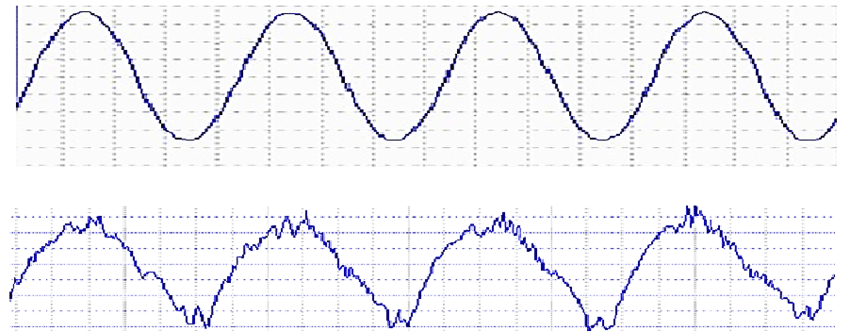
\includegraphics[width=\textwidth]{img/Distortion.png}
			\end{figure}
		\end{itemize}
	
	
	L'information est représentée sous la forme d'un signal. Cela veut dire que changer l'amplitude du signal ne change pas l'information. Mais la distorsion elle change l'information car le signal change de forme et donc modification du signal et de l'information.
	
\subsubsection*{3 moyens de représenter le signal :}
	\begin{itemize}
		\item \textbf{Signaux analogiques}
		\item \textbf{Signaux numériques}
		\item \textbf{Numérisation} : Transformation de signaux analogique en numérique.
	\end{itemize}
		\begin{figure}[H]
			\centering
			\includegraphics[width=0.6\textwidth]{img/Analogique-Numérique.png}
		\end{figure}
		
	\subsection{Transformation de Fourier}
		Moyen de représenter un signal par un ensemble de fréquence. Elle permet d'analyser un signal en une somme de sinusoïde = \textbf{Contenu fréquentiel}.
		\begin{figure}[H]
			\centering
			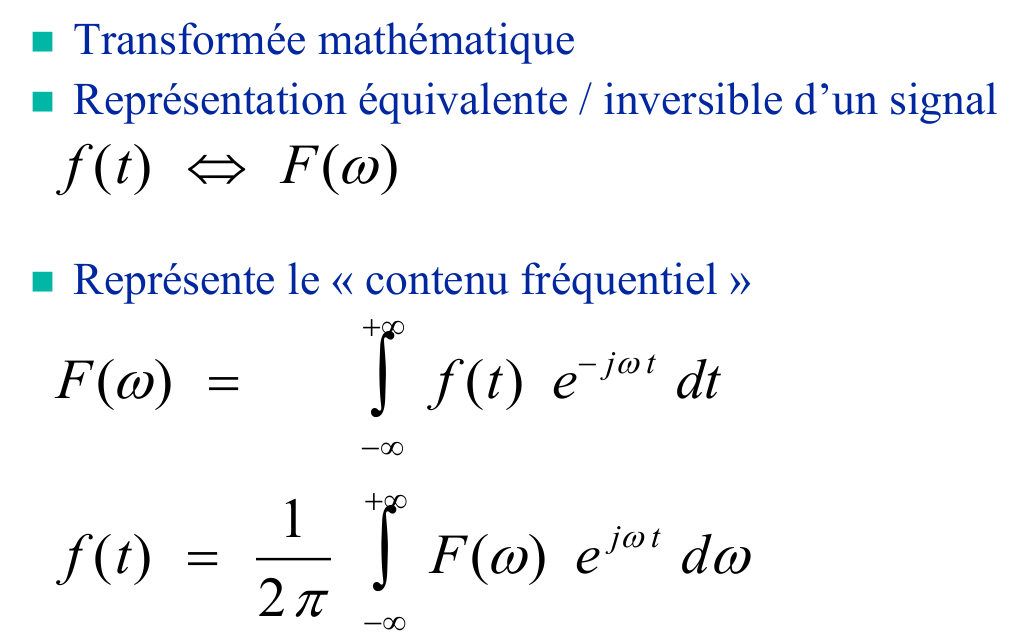
\includegraphics[width=0.6\textwidth]{img/Fourrier.png}
			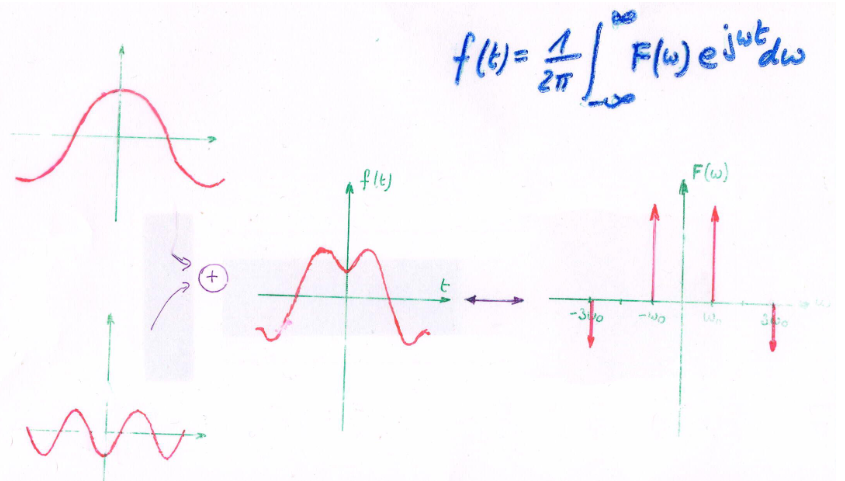
\includegraphics[width=0.6\textwidth]{img/FourrierExemple.png}
		\end{figure}
		
		On peut voir sur les schémas que la fonction $f(t)$ est la somme des 2 sinusoïdes dans l'exemple donné. Mais la fonction $F(\omega)$, si on ne regarde que du coté positif, $F(\omega)$ représente qu'il y a une sinusoïde à 10kHz (première flèche vers le haut) et un sinusoïde à 30kHz, celle-ci pointe vers le bas car elle commence à un nombre négatif sur le schéma.
		
	\subsection{Bande de Fréquence}
		Tous les systèmes de télécom sont limités en fréquence = la bande de fréquence du système.
		
		La \textbf{Modulation} permet de transposer un signal autour d'un fréquence définie, c'est utilisé pour partager les différentes bandes de fréquence.
		
		Un signal \textbf{modulé} est un signal \textbf{modulant} mis sur une \textbf{porteuse} à la fréquence désirée.
		
		Le \textbf{Multiplexage} permet de faire passer plusieurs informations sur un seul support de fréquence. Les différents symboles sont combinés grâce à un multiplexeur. Deux types:
		\begin{itemize}
			\item \textbf{Temporel}
			\item \textbf{Fréquentiel}
		\end{itemize}
		\begin{figure}[H]
			\centering
			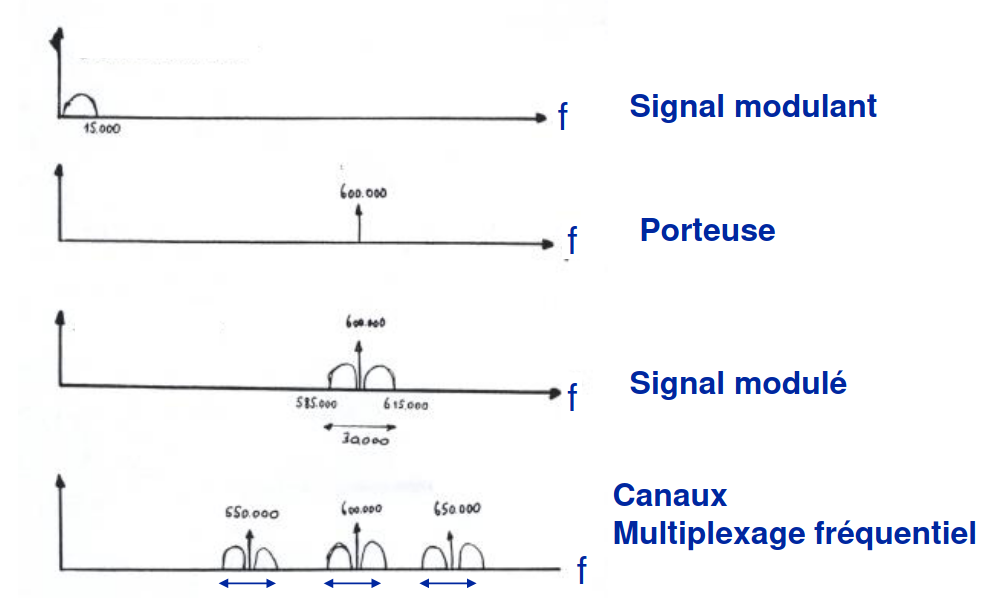
\includegraphics[width=0.6\textwidth]{img/Multiplexage.png}
		\end{figure}
	\subsection{Exemples}
		\subsubsection{Son}
			Un micro capture les ondes de pressions dûes à la voix sous la forme d'un signal électrique.
			
			Le haut-parleur lui reçoit le signal électrique et fait vibrer une membrane pour recréer le son.
			
			
		\subsubsection{Stéréo}
		
			Les sons gauches (G) et droites (D) sont envoyés ensemble sous un signal $S_1 = G+D$ donc la somme des 2. Grâce à ça les radios Mono peuvent recevoir le signal aussi. Un autre signal est aussi envoyé par la stéréo : $S_2 = G-D$. Le signal stéréo peut alors être recréé avec l'opération suivante


			\begin{align*} 
				G &=  S_1 + S2 = (G+D) + (G-D) = 2G \\ 		
				D &=  S_1 - S2 = (G+D) - (G-D) = 2D
			\end{align*}
			
			On va avoir un effet de compression car $S_2$ est souvent très petit par rapport à $S_1$. $S_2$ a un contenu fréquentiel faible et aura donc une bande de fréquence plus faible.
		
		\subsubsection{TV analogique}
		
			On joue sur la luminance (niveau de gris) des lignes est envoyée par pulsation de synchronisation (Synchronizing pulse) entre chaque ligne.

			Un canon à électrons envoie la lumière ligne après ligne sur l'écran pour afficher une image
			
\begin{figure}[H]
\centering
\begin{minipage}{.5\textwidth}
  \centering
  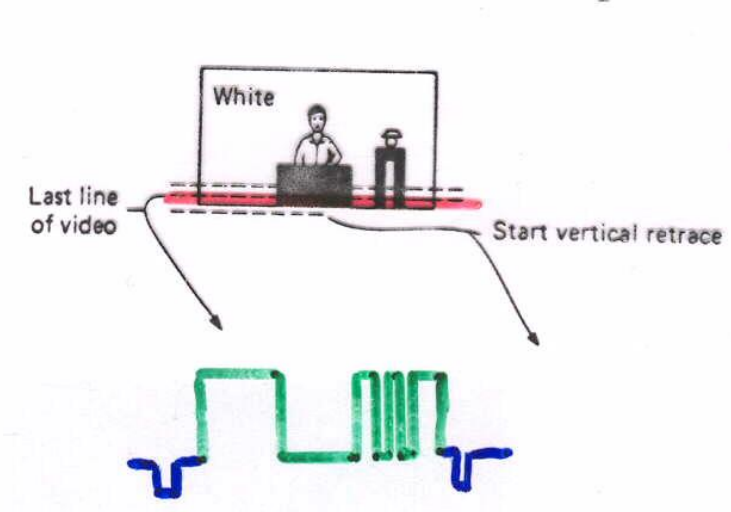
\includegraphics[width=.5\textwidth]{img/TV1.png}
\end{minipage}%
\begin{minipage}{.5\textwidth}
  \centering
  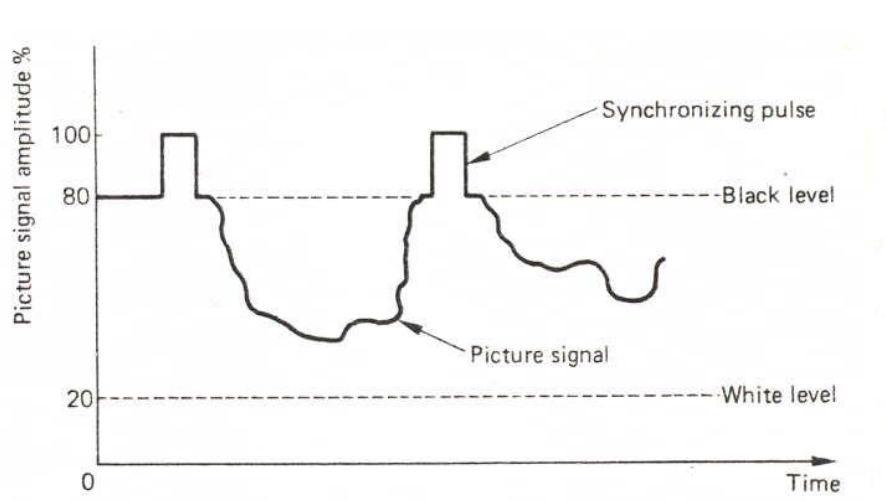
\includegraphics[width=.5\textwidth]{img/TV2.png}
\end{minipage}
\end{figure}
			
			Pour les couleurs, on fait pareil que la stéréo, on garde l'envoi de luminance pour que les vieilles TVs fonctionnent encore.
			
			On a donc \textit{RGB} (red,green,blue) et \textit{YUV} les signaux (luminance Y et chrominance U V)
			
			\begin{align*} 
				Y &= 0.3\textcolor{red}{R} + 0.59\textcolor{green}{G} + 0.11\textcolor{blue}{B}\\
				U &= 0.493(\textcolor{blue}{B}-Y)\\
				V &= 0.877(\textcolor{red}{R}-Y)
			\end{align*}
	\subsection{Signaux numérique}
		C'est simple, c'est du binaire.
		
		Si on a un signal analogique et que on veut en faire un numérique $\rightarrow$ Numérisation.
		
		Il peut y avoir des erreurs dans ce que on a transmis et ce que on lit.
		
	\subsection{Numérisation}
		Passer d'un signal analogique à un signal numérique. On va devoir \textbf{Échantillonner} le signal (captures de valeur à intervalles fixes). Car le signal numérique a des avantages :
		\begin{itemize}
			\item Traitement et stockage de l'information.
			\item Regénération du signal par des codes correcteurs et détecteurs d'erreur.
		\end{itemize}
		
		Signal analogique représenté par des valeurs continues ($\mathbb{R}$) et signal numérique par des valeurs discrètes (0 ou 1).
		
		Le procédé de transformation est appelé \textbf{Quantification}, on remplace les valeurs continues reçues par les valeurs discrètes qui s'en rapprochent le plus.
		
		Avantage du numérique est que le bruit dans l'analogique sera filtré s'il est faible.
		
		Lors de l'échantillonnage, il ne faut pas prendre une fréquence trop grande sous peine d'avoir beaucoup d'erreur. Le \textbf{Théorème de Shannon} certifie que il n'y a aucune perte si la fréquence d'échantillonnage est au moins 2 fois supérieure à la fréquence maximum du signal.
		
		\begin{figure}[H]
			\centering
			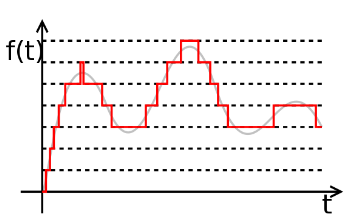
\includegraphics[width=0.6\textwidth]{img/Quantification.png}
		\end{figure}		
		
		
		